\documentclass{report}
    \title{50004 - Operating Systems - Lecture 3}
    \author{Oliver Killane}
    \date{21/10/21}

%===========================COMMON FORMAT & COMMANDS===========================
% This file contains commands and format to be used by every module, and is 
% included in all files.
%===============================================================================

%====================================IMPORTS====================================
\usepackage[a4paper, total={6in, 8in}]{geometry}
\usepackage{graphicx, amssymb, amsfonts, amsmath, xcolor, listings, tcolorbox, multirow, hyperref}
%===============================================================================

%====================================IMAGES=====================================
\graphicspath{{image/}}

% \centerimage{options}{image}
\newcommand{\centerimage}[2]{\begin{center}
    \includegraphics[#1]{#2}
\end{center}}
%===============================================================================

%=================================CODE LISTINGS=================================
\definecolor{codebackdrop}{gray}{0.9}
\definecolor{commentgreen}{rgb}{0,0.6,0}
\lstset{
    inputpath=code, 
    commentstyle=\color{commentgreen},
    keywordstyle=\color{blue}, 
    backgroundcolor=\color{codebackdrop}, 
    basicstyle=\footnotesize,
    frame=single,
    numbers=left,
    stepnumber=1,
    showstringspaces=false,
    breaklines=true,
    postbreak=\mbox{\textcolor{red}{$\hookrightarrow$}\space}
}

% Create a code listing for a single line
% \codeline{language}{line}{file}
\newcommand{\codeline}[3]{\lstinputlisting[language=#1, firstline = #2, lastline = #2]{#3}}

% Create a code listing for a given language & file
% \codelist{language}{file}
\newcommand{\codelist}[2]{\lstinputlisting[language=#1]{#2}}
%===============================================================================

%================================TEXT STRUCTURES================================
% Marka a word as bold
% \keyword{important word}
\newcommand{\keyword}[1]{\textbf{#1}}

% Creates a section in italics
% \question{question in italics}
\newcommand{\question}[1]{\textit{#1} \\ }

% Creates a box with title for side notes.
% \sidenote{title}{contents}
\newcommand{\sidenote}[2]{\begin{tcolorbox}[title=#1]#2\end{tcolorbox}}

% Creates an item in an itemize or enumerate, with a paragraph after
% \begin{itemize}
%     \bullpara{title}{contents}
% \end{itemize}
\newcommand{\bullpara}[2]{\item \textbf{#1} \ #2}

% Creates a compact list (very small gaps between items)
% \compitem{
%     \item item 1
%     \item item 2
%     \item ...
% }
\newcommand{\compitem}[1]{\begin{itemize}\setlength\itemsep{-0.5em}#1\end{itemize}}

% Creates a link to the lecture for use at the start of the notes document
\newcommand{\lectlink}[1]{\sidenote{Lecture Recording}{
    Lecture recording is available \href{#1}{here}
}}
%===============================================================================


%==============================SYNTAX HIGHLIGHTING==============================
\newcommand{\fun}[1]{\textcolor{blue}{\textbf{#1}}}
\newcommand{\file}[1]{\textcolor{green}{\textbf{#1}}}
\newcommand{\struct}[1]{\textcolor{orange}{\textbf{#1}}}
\newcommand{\var}[1]{\textcolor{purple}{\textbf{#1}}}
\newcommand{\const}[1]{\textcolor{red}{\textbf{#1}}}
%===============================================================================

%==============================THREAD HIGHLIGHTING==============================
\newcommand{\threada}[1]{\textcolor{green}{\textbf{#1}}}
\newcommand{\threadb}[1]{\textcolor{red}{\textbf{#1}}}
%===============================================================================

%============================DISPLAYING THREAD CODE=============================
\newcommand{\threadlist}[3]{
    \codelist{#1}{#2 init.#3}
    \begin{minipage}[t]{0.45\textwidth}
        \codelist{#1}{#2 A.#3}
    \end{minipage}
    \hfill
    \begin{minipage}[t]{0.45\textwidth}
        \codelist{#1}{#2 B.#3}
    \end{minipage}
}
%===============================================================================

\begin{document}
\maketitle
\sidenote{Lecture Recording}{
	Lecture recording is available \href{https://imperial.cloud.panopto.eu/Panopto/Pages/Viewer.aspx?id=3481ee11-1caf-482d-9f1e-adc600ce0ec0}{here}
}

\section*{Threads}
Threads are execution streams that share the same address space. When multi-threading is used, each process can have more than one thread.
\begin{center}
	\begin{tabular}{r l}
		\keyword{Process} & \keyword{Thread} \\
		Address Space     & Program Counter  \\
		Global Variables  & Registers        \\
		Open files        & Stack            \\
		Child Processes                      \\
		Signals                              \\
	\end{tabular}
\end{center}

Applications may want to run many activities in parallel, with access shared memory. They also need to be capable of synchronisation, through semaphores, locks \& monitors or blocking to prevent race conditions on shared data.
\\
\\ Processes have several disadvantages:
\begin{itemize}
	\bullpara{Communication}{
		\\ Difficult to communicate between different address spaces, requiring system calls (which have overhead if a context switch is required).
		\\
		\\ If we split our program into several processes, each has a different address space, so all communication (internally in our program) has to use expensive system calls.
	}
	\bullpara{Blocking}{
		\\ Blocking activities may block the whole process, rather than one thread of a process.
	}
	\bullpara{Context Switches}{
		\\ Transfering between processes requires expensive context switches.
	}
	\bullpara{Create \& Kill}{
		\\ Creation and desruction costs are higher.
	}
\end{itemize}
Threads are a more lightweight abstraction for concurrency.
\\
\\ However threads access shared data, which means race conditions \& memory corruption can occur.
\section*{PThreads}
\lstinputlisting[language=C]{pthread.c}
Defined by \keyword{IEEE} standard 1003.1c and implemented on most \keyword{UNIX} systems. A library that internally makes systems calls to enable threading.
\lstinputlisting[language=C]{pthread.c}

\subsubsection*{Creating Threads}
\lstinputlisting[language=C, firstline=1, lastline=1]{thread declarations.c}
Creates a new thread stored in \struct{thread}, returning $0$ for a successful creation, or an error code for failure.
\\
\\ Arguments:
\begin{itemize}
	\bullpara{attr}{
		\\ specifies thread attributes, can be \const{NULL} for default (e.g minimum stack stack size, guard size, detached/joinable etc)
	}
	\bullpara{start\_routine}{
		\\ C function the thread will start executing from, returning some pointer, and taking some pointer as arguments.
	}
	\bullpara{arg}{
		\\ Arguments to be passed to start routine, can be \const{NULL} if no arguments are to be passed.
	}
\end{itemize}
\subsubsection*{Terminating Threads}
\lstinputlisting[language=C, firstline=2, lastline=2]{thread declarations.c}
Terminates the thread and makes \struct{value\_ptr} available to any successful join with the terminating thread.
\\
\\ Is called implicitly when the thread's start routine returns.
\begin{itemize}
	\item Not called for the initial thread (that started main).
	\item If \fun{main} terminates before other threads without calling \fun{pthread\_exit}, the entire process is terminated.
	\item If \fun{pthread\_exit} is called in \fun{main} the process continues executing until the last thread terminates (or \fun{exit} is called.).
\end{itemize}
\lstinputlisting[language=C]{pthread example.c}

\subsubsection*{Yielding Thread}
\lstinputlisting[language=C, firstline = 3, lastline = 3]{thread declarations.c}
Releases the \keyword{CPU} to let another thread run. Returns $0$ on success. In linux it always succeeds.

\subsubsection*{Joining Threads}
\lstinputlisting[language=C, firstline=4, lastline=4]{thread declarations.c}
Blocks until the thread terminates. The value passed to \fun{pthread\_exit} is available on location referenced by \struct{value\_ptr} (can be \const{NULL}) for example an error value may be propagated.
\lstinputlisting[language=C]{pthread join example.c}

\section*{OS Thread Implementation}
The two main  approaches are \keyword{User-Level Threads} and \keyword{Kernel-Level Threads}. Both have tradeoffs and hybrid approaches are possible.

\subsubsection*{User Level Threads}
OS Kernel is manages processes only. Threads are implemented through a library, with running processes maintaining their own thread table to manage their threads.
\begin{center}
	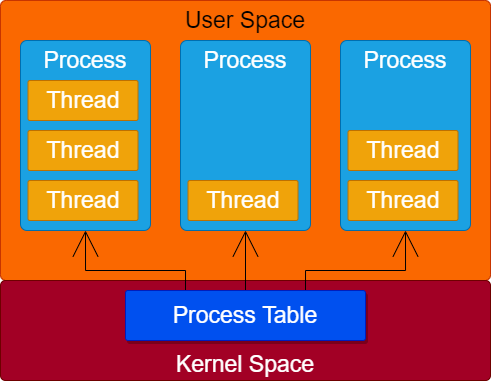
\includegraphics[width=0.5\textwidth]{user level threads.png}
\end{center}
\textbf{Advantages}
\begin{itemize}
	\bullpara{Better Performance}{
		\\As the kernel is not involved in thread creation, termination, switching or synchronisation. They can be much faster.
		\\
		\\ Fewer expensive context switches as less kernel involvement.
	}
	\bullpara{Optimisation}{
		\\ Each application can have its own scheduling algorithm, which can be optimised for the specific context of that application. Which aides performance.
	}
\end{itemize}
\textbf{Disadvantages}
\begin{itemize}
	\bullpara{Blocking Calls}{
		A blocking system call blocks the process (and all threads inside), which denies a key motivation for using threads.
		\\
		\\ While non-blocking I/O can be used (e.g \fun{select}) they are more complex \& inelegant.
	}
	\bullpara{Exceptions}{
		\\ Exceptions can block all threads, even if some are runnable (e.g page-fault).
	}
\end{itemize}
\sidenote{Select}{
	\fun{select} and \fun{pselect} allow a program to monitor multiple file descriptors, waiting for some to become ready for some I/O before doing it.
	\begin{center}
		\begin{minipage} {0.8\textwidth}
			\lstinputlisting[language=C]{select example.c}
		\end{minipage}
	\end{center}
}
\subsubsection*{Kernel Level Threads}
The OS kernel manages the threads of processes directly.
\begin{center}
	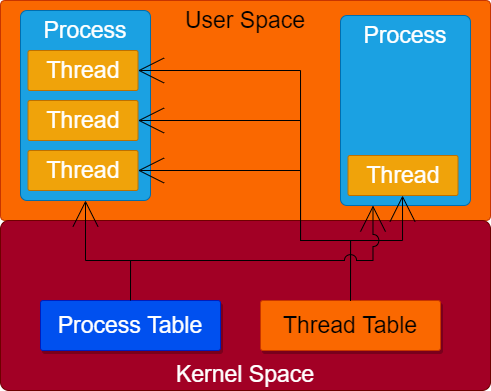
\includegraphics[width=0.5\textwidth]{kernel level threads.png}
\end{center}
\textbf{Advantages}
\begin{itemize}
	\bullpara{Blocking Calls}{
		\\ Blocking calls \& exceptions (e.g page fault) do not block whole process, if one thread in a process is blocked, the kernel can schedule another runnable thread from that process.
	}
\end{itemize}
\textbf{Disadvantages}
\begin{itemize}
	\bullpara{Thread Creation more expensive}{
		\\ Requires systemn calls (though is still cheaper than creating a new process).
		\\
		\\ A mitigation stragetgy is to use thread pools (recycling threads).
	}
	\bullpara{Synchronisation}{
		\\ Requires blocking system calls, which are expensive.
	}
	\bullpara{Switching more expensive}{
		\\ Requires a system call, kernel the schedule. Kernel scheduler be optimal for all applications (however still cheaper than switching processes).
	}
	\bullpara{No application-specific Schedulers!}{}
\end{itemize}
\subsubsection*{Hybrid Approaches}
A suggested hybrid approach is to map user level threads, to a lower number of kernel threads. This has some of the advantages of both approaches, however requires some overhead in creating the mapping, and updating it.
\begin{center}
	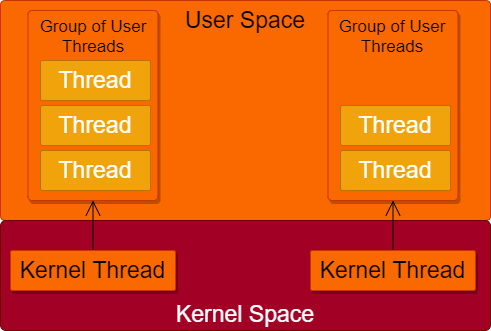
\includegraphics[width=0.5\textwidth]{hybrid threads.png}
\end{center}
The user level threads do not have 'real' concurrency in this approach, only kernel threads.
\end{document}
